\chapter{El MC-TTRP}
En este capítulo se tratarán los problemas de rutas, en específico, se definirá y se dará una expresión formal para el problema de rutas de tráileres y camiones multicompartimento (MC-TTRP por sus siglas en inglés). Este capítulo se basará en los primeros 2 capítulos de la tesis de doctoramiento \cite{laura-mcttrp}
\section{Introducción a los problemas de rutas}
Los problemas de rutas de vehículos (VRP por sus siglas en inglés) son algunos de los problemas más importantes dentro de la optimización combinatoria. Estos problemas buscan, como su nombre indica, encontrar el conjunto de rutas óptimas que deben seguir un conjunto de vehículos para servir a un conjunto de clientes. Los VRP fueron introducidos por primera vez durante la década de los 50 \cite{vrp-og} y nacen como una generalización del problema del viajante de comercio \cite{tsp-dantzig}. Ambos problemas pueden ser vistos como un problema de optimización de un grafo, para los que existen múltiples métodos de resolución exactos. Sin embargo, estos problemas pertenecen a una clase de problemas denominada NP-Duros (ver Anexo \ref{anexoCC}), por lo que el uso de métodos aproximados (como las metaheurísticas) es recomendado.\\

El VRP original consiste en la generación de $n$ rutas tal que se puedan repartir bienes a un conjunto de clientes distribuidos geográficamente cuyas demandas son determinísticas, conocidas de antemano y no divisibles. Además, sólo existe un depósito desde donde todos los vehículos deben partir y regresar. La función objetivo de este tipo de problemas es la minimización de la distancia total recorrida. Se puede ver un ejemplo de un problema de este tipo en la Figura \ref{fig:VRP}.\\

\begin{figure}[!bt]
    \centering
    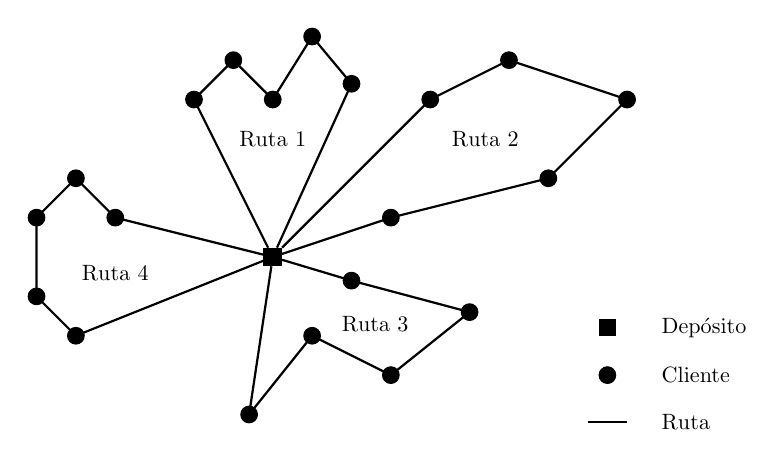
\begin{tikzpicture}[scale=1, every node/.style={scale=0.8}]
        
        % Depot
        \node[draw, fill=black, minimum size=8pt, shape=rectangle] (depot) at (0,0) {};
        
        % Ruta 1
        \coordinate (r1a) at (-1,2);
        \coordinate (r1b) at (-0.5,2.5);
        \coordinate (r1c) at (0,2);
        \coordinate (r1d) at (0.5,2.8);
        \coordinate (r1e) at (1,2.2);
        
        \draw[thick] (depot) -- (r1a);
        \draw[thick] (r1a) -- (r1b) -- (r1c) -- (r1d) -- (r1e) -- (depot);
        \foreach \x in {r1a, r1b, r1c, r1d, r1e} \filldraw[black] (\x) circle (3pt);
        \node at (0,1.5) {Ruta 1};
        
        % Ruta 2
        \coordinate (r2a) at (1.5,0.5);
        \coordinate (r2b) at (3.5,1);
        \coordinate (r2c) at (4.5,2);
        \coordinate (r2d) at (3,2.5);
        \coordinate (r2e) at (2,2);
        
        \draw[thick] (depot) -- (r2a);
        \draw[thick] (r2a) -- (r2b) -- (r2c) -- (r2d) -- (r2e) -- (depot);
        \foreach \x in {r2a, r2b, r2c, r2d, r2e} \filldraw[black] (\x) circle (3pt);
        \node at (2.7,1.5) {Ruta 2};
        
        % Ruta 3
        \coordinate (r3a) at (1,-0.3);
        \coordinate (r3b) at (2.5,-0.7);
        \coordinate (r3c) at (1.5,-1.5);
        \coordinate (r3d) at (0.5,-1);
        \coordinate (r3e) at (-0.3,-2);
        
        \draw[thick] (depot) -- (r3a);
        \draw[thick] (r3a) -- (r3b) -- (r3c) -- (r3d) -- (r3e) -- (depot);
        \foreach \x in {r3a, r3b, r3c, r3d, r3e} \filldraw[black] (\x) circle (3pt);
        \node at (1.3,-0.85) {Ruta 3};
        
        % Ruta 4
        \coordinate (r4a) at (-2,0.5);
        \coordinate (r4b) at (-2.5,1);
        \coordinate (r4c) at (-3,0.5);
        \coordinate (r4d) at (-3,-0.5);
        \coordinate (r4e) at (-2.5,-1);
        
        \draw[thick] (depot) -- (r4a);
        \draw[thick] (r4a) -- (r4b) -- (r4c) -- (r4d) -- (r4e) -- (depot);
        \foreach \x in {r4a, r4b, r4c, r4d, r4e} \filldraw[black] (\x) circle (3pt);
        \node at (-2,-0.2) {Ruta 4};
        
        % Legend
        \begin{scope}[xshift=4cm, yshift=-1cm]
          \draw[fill=black] (0.15,0) rectangle +(0.2,0.2);
          \node[right=0.3cm] at (0.6,0.1) {Depósito};
          \filldraw[black] (0.25,-0.5) circle (3pt);
          \node[right=0.3cm] at (0.6,-0.5) {Cliente};
          \draw[thick] (0,-1.1) -- (0.5,-1.1);
          \node[right=0.3cm] at (0.6,-1.1) {Ruta};
        \end{scope}
        
    \end{tikzpicture}
    \caption{Posible solución de un VRP. En esta solución se tienen $n$ vehículos.}
    \label{fig:VRP}
\end{figure}

Aparte de los problemas de rutas básicos, existen diversas variaciones. Cada variación cambia algún parámetro del problema o añade algún tipo de restricción. Por ejemplo, la demanda puede ser estocástica (VRPSD), pueden existir múltiples depósitos (MDVRP), pueden añadirse ventanas temporales (VRPTW), etc. El problema que nos concierne, el MC-TTRP, nace de la combinación de dos variaciones del problema de rutas:
\begin{itemize}
    \item Problema de rutas con múltiples compartimentos (MC-VRP). La demanda de los clientes se encuentra en múltiples compartimentos que no se pueden mezclar.
    \item Problema de rutas con restricciones de accesibilidad. Existen varios tipos de vehículos, y cada vehículo puede acceder a un tipo específico de rutas.
\end{itemize}

Además de estas variantes, también se tendrán en cuenta otras restricciones extra como la capacidad máxima de transporte. Veamos cómo se define este problema.

\section{Definición formal del MC-TTRP}
Como se indicaba anteriormente, el problema a tratar es el problema de rutas de camiones y tráileres multicompartimento (MC-TTRP) basado en el problema de rutas de camiones y tráileres (TTRP por sus siglas en inglés, \cite{chao-ttrp}). En este problema se añaden restricciones de accesibilidad y 2 tipos de vehículos: camiones y camiones cargando un tráiler. Existen 2 tipos de clientes: aquellos a los que se puede acceder con el camión cargando un tráiler ($VC$) y aquellos a los que solo se puede acceder con un camión sin carga ($TC$). Si pensamos en la aplicación de este problema al mundo real, se ve que los $TC$ son aquellos clientes en centros de ciudades, regiones montañosas o pequeños pueblos, en los cuales no se puede maniobrar un tráiler completo. Los VC son el resto de los clientes. Para resolver este problema se definen 3 tipos de rutas:
\begin{itemize}
    \item Rutas de camión ($RC$): Aquellas rutas que solo pueda circular un camión sin tráiler.
    \item Rutas de tráileres ($RT$): Aquellas rutas por las que pueda circular un vehículo completo (camión remolcando un tráiler).
    \item Rutas mixtas ($RM$): Estas rutas consisten de una ruta principal del tipo $RT$, pero que incluye subrutas de tipo $RC$. En este tipo de rutas el tráiler es aparcado en una de las localizaciones y sólo el camión recorre la subruta $RC$.
\end{itemize}
Podemos ver un ejemplo de una solución para un problema de este estilo en la Figura \ref{fig:TTRP}.

\begin{figure}
    \centering
    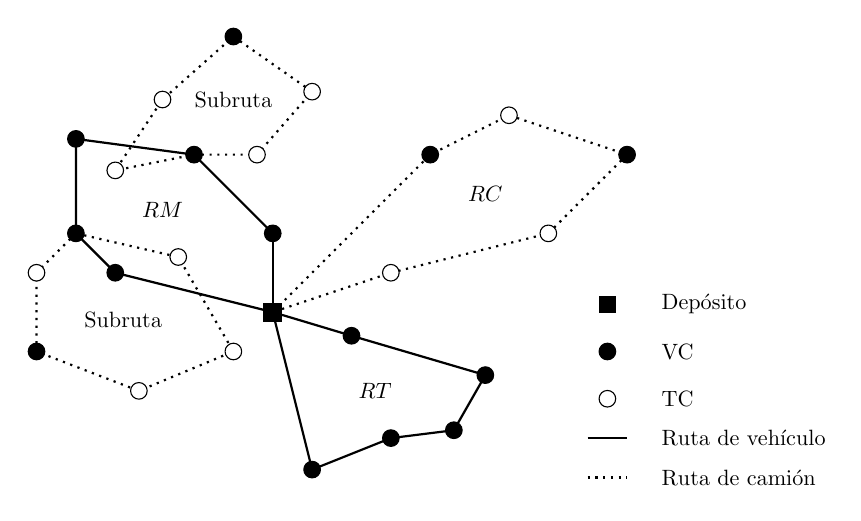
\begin{tikzpicture}[scale=1, every node/.style={scale=0.8}]
        
        % Depot
        \node[draw, fill=black, minimum size=8pt, shape=rectangle] (depot) at (0,0) {};
        
        
        
        % Ruta 2
        \coordinate (r2a) at (1.5,0.5);
        \coordinate (r2b) at (3.5,1);
        \coordinate (r2c) at (4.5,2);
        \coordinate (r2d) at (3,2.5);
        \coordinate (r2e) at (2,2);
        
        \draw[thick,dotted] (depot) -- (r2a);
        \draw[thick,dotted] (r2a) -- (r2b) -- (r2c) -- (r2d) -- (r2e) -- (depot);
        \foreach \x in {r2c, r2e} \filldraw[black] (\x) circle (3pt);
        \filldraw[fill=white, draw=black] (r2a) circle (3pt);
        \filldraw[fill=white, draw=black] (r2b) circle (3pt);
        \filldraw[fill=white, draw=black] (r2d) circle (3pt);
        \node at (2.7,1.5) {$RC$};
        
        % Ruta 3
        \coordinate (r3a) at (1,-0.3);
        \coordinate (r3b) at (2.7,-0.8);
        \coordinate (r3c) at (2.3,-1.5);
        \coordinate (r3d) at (1.5,-1.6);
        \coordinate (r3e) at (0.5,-2);
        
        \draw[thick] (depot) -- (r3a);
        \draw[thick] (r3a) -- (r3b) -- (r3c) -- (r3d) -- (r3e) -- (depot);
        \foreach \x in {r3a, r3b, r3c, r3d, r3e} \filldraw[black] (\x) circle (3pt);
        \node at (1.3,-1) {$RT$};
        
        % Ruta 4
        
        
        
        % \draw[thick] (depot) -- (r4a);
        % \draw[thick] (r4a) -- (r4b) -- (r4c) -- (r4d) -- (r4e) -- (depot);
        % \foreach \x in {r4a, r4b, r4c, r4d, r4e} \filldraw[black] (\x) circle (3pt);
        % \foreach \x in {r4c,r4d,r4e} \filldraw[fill=white, draw=black] (\x) circle (3pt);
        % \node at (-2,-0.2) {Ruta 4};

        % Ruta 1
        \coordinate (r1a) at (-1,2);
        \coordinate (r1c) at (0,1);        
        \coordinate (r1e) at (-2.5,2.2);
        \coordinate (r4a) at (-2,0.5);
        \coordinate (r4b) at (-2.5,1);

        % Subroute 1
        \coordinate (st1a) at (-0.2,2);
        \coordinate (st1b) at (0.5,2.8);
        \coordinate (st1c) at (-0.5,3.5);
        \coordinate (st1d) at (-1.4,2.7);
        \coordinate (st1e) at (-2,1.8);

        % Subroute 2
        \coordinate (st2a) at (-3,0.5);
        \coordinate (st2b) at (-3,-0.5);
        \coordinate (st2c) at (-1.7,-1);
        \coordinate (st2d) at (-0.5,-0.5);
        \coordinate (st2e) at (-1.2,0.7);
        
        \draw[thick] (depot) -- (r1c);
        \draw[thick] (r1c) -- (r1a) -- (r1e) -- (r4b) -- (r4a) -- (depot);
        \draw[thick,dotted] (r1a) -- (st1a) -- (st1b) -- (st1c) -- (st1d) -- (st1e) -- (r1a);
        \draw[thick,dotted] (r4b) -- (st2a) -- (st2b) -- (st2c) -- (st2d) -- (st2e) -- (r4b);
        \foreach \x in {r1c, r1a, r1e, r4b, r4a, st1c, st2b} \filldraw[black] (\x) circle (3pt);
        \foreach \x in {st2a,st2c,st1a,st1b,st1d,st1e,st2d,st2e} \filldraw[fill=white, draw=black] (\x) circle (3pt);
        \node at (-0.5,2.7) {Subruta};
        \node at (-1.9,-0.1) {Subruta};
        \node at (-1.4,1.3) {$RM$};
        
        % Legend
        \begin{scope}[xshift=4cm, yshift=-0cm]
          \draw[fill=black] (0.15,0) rectangle +(0.2,0.2);
          \node[right=0.3cm] at (0.6,0.1) {Depósito};
          \filldraw[black] (0.25,-0.5) circle (3pt);
          \node[right=0.3cm] at (0.6,-0.5) {VC};
          \draw[black] (0.25,-1.1) circle (3pt);
          \node[right=0.3cm] at (0.6,-1.1) {TC};
          \draw[thick] (0,-1.6) -- (0.5,-1.6);
          \node[right=0.3cm] at (0.6,-1.6) {Ruta de vehículo};
          \draw[thick,dotted] (0,-2.1) -- (0.5,-2.1);
          \node[right=0.3cm] at (0.6,-2.1) {Ruta de camión};

          
        \end{scope}
        
    \end{tikzpicture}
    \caption{Posible solución de un problema TTRP.}
    \label{fig:TTRP}
\end{figure}

El segundo problema que añade el MC-TTRP es el problema de rutas multicompartimento. Esta nueva restricción indica que tanto los tráileres como los camiones tendrán múltiples compartimentos que no se pueden mezclar y con una capacidad máxima independiente. Veamos la formulación formal de este problema como un modelo de programación lineal en enteros mixta (PLEM).

\subsection{Modelo PLEM para el MC-TTRP}
Como se indica anteriormente, el modelo que se propone es un modelo de programación lineal en enteros mixta, y se utilizará una versión simplificada de aquel dado por \cite{laura-mcttrp}, donde se eliminan las restricciones de tiempo y aquellas relacionadas con la carga máxima legal.\\

Este problema puede ser descrito de la siguiente manera. Sea $G=(N,E)$ un grafo no dirigido formado por un conjunto de nodos $N=\{0,1,\ldots,n\}$, que representan el depósito ($0$) y a los clientes ($1,\ldots,n$), y un conjunto $E=\{(i,j)\in N\times N\;|\;i\neq j\}$ que representa los ejes que unen los nodos. Se tiene que $N_1, N_2\subset N$ tal que $N_1$ contiene los $n_1$ nodos que corresponden a los $VC$ y $N_2$ contiene los $n-n_1$ nodos correspondientes a los $TC$. Para cada elemento $(i,j)\in E$ se asigna un coste no negativo $c_{ij}$, que representa la distancia entre los nodos $i$ y $j$. Para realizar el transporte se definen dos conjuntos: un conjunto $K^T=\{1,\ldots,m_L,\ldots,m_T\}$ de camiones y un conjunto $K^L=\{1,\ldots,m_L\}$ de tráileres. Para el primer conjunto se definen 2 subconjuntos: $K^T_1=\{1,\ldots,m_L\}$ y $K_2^T=\{m_L+1,\ldots,m_T\}$; que representan aquellos camiones que puedan remolcar un tráiler y aquellos que no respectivamente. Para estos conjuntos anteriores, se tiene que $m_l$ es el número de tráileres y $m_t$ el número de camiones ($m_l\leq m_t$), y todos los vehículos se consideran homogéneos. Se definen como $Q_T$ y $Q_L$ la capacidad de cada camión y cada tráiler respectivamente. Por consiguiente, la capacidad de un vehículo completo se define como $Q_T+Q_L$.\\

Como se menciona al inicio de esta sección, y se observa en la Figura \ref{fig:TTRP}, existen 3 tipos de caminos posibles. Para las $RM$, el camino que realiza el vehículo completo se denomina ruta principal. Durante el recorrido del camino principal, es posible desacoplar el tráiler y dejarlo aparcado en un parking (un parking puede ser cualquier VC o incluso el depósito). Las subrutas comienzan y terminan en un parking de la ruta pricipal de la $RM$. Dentro de una subruta es posible servir a cualquier tipo de cliente. No existen restricciones en el número máximo de subrutas que puede tener una $RM$, ni tampoco en el número máximo de subrutas distintas que pueden comenzar desde el mismo parking, en el caso de que se satisfagan las restricciones de capacidad. Esto significa que la demanda de una $RM$ no puede exceder la capacidad de un vehículo completo ($Q_T+Q_L$), y $Q_T$ no puede ser sobrepasado en ninguna subruta. Para las $RT$, que solo pueden abastecer a los $VC$, la restricción que existe es que la demanda no puede ser mayor a la capacidad del vehículo completo. De manera similar, para las $RC$, que pueden abastecer a ambos tipos de clientes, la demanda de la ruta deberá ser inferior a la capacidad del camión $Q_T$.\\

% Me quede en el tercer párrafo:
% For the sake of simplicity, it is also assumed that travel costs are the same for all
Para mayor simplicidad, se supone que el coste de los viajes es el mismo para cualquier vehículo. Cada tráiler $r\in K^L$ está dividido en compartimentos, $H^L$, donde $Q_L^H$ representa la capacidad de los compartimento. Análogamente, cada camión $k\in K^T$ se divide en un conjunto de compartimentos $H^T$, y $Q_T^H$ representa las capacidades. Estos compartimentos (que no se pueden mezclar y deben servir únicamente a un cliente) sirven para dividir los distintos tipos de carga representados por el conjunto $F=\{1,\ldots,n_F\}$. Cada nodo (menos el depósito) tiene una demanda no negativa $d_{if}$ $(i\in N\setminus\{0\}=N^*,f\in F)$ por cada tipo de carga. La demanda de cada cliente deberá ser cumplida por un único vehículo y es posible cumplir la demanda utilizando múltiples compartimentos del mismo tipo de carga.\\

Con respecto a las variables de decisión del modelo, $x_{ij}^{kr}$ y $y_{ij}^{klv}$ (ambas binarias) están relacionadas con la construcción de rutas. La primera variable está relacionada con las rutas recorridas por un vehículo completo, y toma el valor $1$ si el camión $k\in K^T$ con el tráiler $r\in K^L$ pasa por el eje $(i,j)$; 0 si no. De manera similar, la segunda variable se relaciona con las rutas recorridas por un camión, tomando el valor $1$ si el camión $k\in K^T$ pasa por el eje $(i,j)$ en la ruta $v\in\mathcal{V}=\{1,\ldots,n\}$ con lugar de parking $l\in N_1\cup\{0\}=N_0^1$; 0 si no. En caso de aparcar en el depósito ($l=0$), el tipo de ruta se considerará $RC$. En otro caso, la variable hará referencia a una subruta de una $RM$. El resto de las variables empleadas por el modelo están relacionadas con los distintos compartimentos. En particular, $ZT^k_{i,f,ht}\in[0,1]$ representa la proporción del compartimento $ht\in H^T$ del camión $k\in K^T$ que lleva la carga $f\in F$ para el cliente $i\in N^*$, mientras que $U_{i,f,ht}^k$ es una variable binaria que toma el valor $1$ si $ZT^k_{i,f,ht}>0$ y 0 si no. Análogamente, se tiene que las variables $ZL^k_{i,f,hl}$ y $V_{i,f,hl}^k$ son el equivalente para los tráileres. Todas estas variables y notaciones se encuentran resumidas en el Cuadro \ref{tab:notation}.\\

El MC-TTRP trata de determinar un conjunto de rutas que minimice el coste total de los ejes viajados tal que se cumplan todas las restricciones, como puede ser que se cumplan las demandas, que no se mezclen mercancías o que no se excedan las capacidades máximas. Veamos como utilizando esta notación podemos expresar el problema como un PLEM:

\begin{table}[t]
\centering
\caption{Notación para el MC-TTRP.}
\label{tab:notation}
\scriptsize
\resizebox{\textwidth}{!}{%
\begin{tabular}{llll}
\hline
\textbf{Conjuntos/parámetros} & \textbf{Definición} & \textbf{Parámetros} & \textbf{Definición} \\ \hline
$\{0\}$ & Depósito & $n$ & Cantidad total de clientes \\
$N_1$ & Conjunto de los VC & $n_1$ & Cantidad de los VC \\
$N_2$ & Conjunto de los TC & $m_L$ & Cantidad de tráileres \\
$N = \{0\} \cup N_1 \cup N_2$ & Conjunto de los nodos & $m_T$ & Cantidad de camiones \\
$N^* = N \setminus \{0\}$ & Conjunto de los clientes & $c_{ij}$ & Distancia de $i$ a $j$ \\
$N_0^1 = N_1 \cup \{0\}$ & Conjunto de los VC y el depósito & $n_F$ & Cantidad de cada tipo de carga \\
$K_1^T$ & Camiones que pueden cargar un tráiler & $d_{if}$ & Demanda del cliente $i$ de la carga $f$ \\
$K_2^T$ & Camiones puros & $Q_T$ & Capacidad de un camión \\
$K^T = K_1^T\cup K_2^T$ & Conjunto de los camiones & $Q_L$ & Capacidad de un tráiler \\
$K^L$ & Conjunto de los tráileres & $Q_T^H$ & Capacidad del compartimento de un camión \\
$F$ & Tipos distintos de carga & $Q_L^H$ & Capacidad del compartimento de un tráiler \\
$H^T$ & Compartimentos del camión & $H^L$ & Compartimentos del tráiler\\
$\mathcal{V}$ & (Sub)Rutas que salen de una raíz & & \\ \hline
\textbf{Variable} & \textbf{Definición} & & \\ \hline
$x_{ij}^{k}$ & \rlap{Variable binaria igual a $1$ si el camión $k$ con el tráiler $r$ pasa por el eje $(i,j)$; 0 si no} & & \\
$y_{ij}^{klv}$ & \rlap{Variable binaria igual a $1$ si el camión $k$ pasa por el eje $(i,j)$ en la (sub)ruta $v$ con parking $l$; 0 si no} & & \\
$U_{i,f,ht}^k$ & \rlap{Variable binaria igual a $1$ si el compartimento $ht$ del camión $k$ lleva la carga $f$ para el cliente $i$; 0 si no} & & \\
$V_{i,f,hl}^r$ & \rlap{Variable binaria igual a $1$ si el compartimento $hl$ del tráiler $r$ lleva la carga $f$ para el cliente $i$; 0 si no} & & \\
$ZT_{i,f,ht}^k$ & \rlap{Proporción del compartimento $ht$ del camión $k$ cargado con la carga $f$ para el cliente $i$} & & \\
$ZL_{i,f,hl}^r$ & \rlap{Proporción del compartimento $hl$ del tráiler $r$ cargado con la carga $f$ para el cliente $i$} & & \\ \hline
\end{tabular}%
}
\end{table}


\allowdisplaybreaks
% Bigass formula
\begin{flalign}
    % Objective function
    &\text{minimizar } \sum_{i\in N_1^0}\sum_{j\in N_1^0}\sum_{k\in K_1^T}\sum_{r\in K^L}c_{ij}x_{ij}^{kr}+\sum_{i\in N}\sum_{j\in N} \sum_{k\in K^T}\sum_{l\in N_1^0}\sum_{v\in \mathcal{V}}c_{ij}y_{ij}^{klv} \label{eq-mcttrp:func-obj}\\
    % No tag
    &\text{sujeto a} \notag \\
    %
    %%%%%%%%%%%%%%%%%%%%% CUSTOMER RESTRICTIONS %%%%%%%%%%%%%%%%%%%%%
    % Each VC must be visited exactly once if it's not a parking spot
    &\sum_{i\in N_1^0}\sum_{k\in K^T_1}\sum_{r\in K^L}x_{ij}^{kr}+\sum_{i\in N}\sum_{k\in K^T}\sum_{\substack{l\in N_1^0 \\ l\neq j}}\sum_{v\in \mathcal{V}}c_{ij}y_{ij}^{klv}=1, & j\in N_1; \label{eq-mcttrp:2.2}\\
    % VC can be present twice if it's the root of a sub-tour
    &\sum_{i\in N_1^0}\sum_{k\in K^T_1}\sum_{r\in K^L}x_{ij}^{kr}+\sum_{i\in N}\sum_{k\in K^T}y_{ij}^{kjv}\leq 2, & \llap{$j\in N_1,v\in \mathcal{V};\;$}\label{eq-mcttrp:2.3}\\
    % TC must be visited only one
    & \sum_{i\in N}\sum_{k\in K^T}\sum_{l\in N_1^0}\sum_{v\in \mathcal{V}}y_{ij}^{klv}=1, & \llap{$j\in N_2$}\label{eq-mcttrp:2.4}\\    
    % Depot cannot be present in any sub-tour
    & \sum_{i\in N}\sum_{k\in K^T}\sum_{l\in N_1}\sum_{v\in \mathcal{V}}y_{ij}^{klv}=0, \label{eq-mcttrp:2.5}\\
    % For each sub-tour or RC the truck goes from the parking spot or the depot to a customer not more than once  
    & \sum_{j\in N}y_{lj}^{klv}\leq 1, & \llap{$k\in K^T;\;l\in N_1^0;\;v\in \mathcal{V};\;$} \label{eq-mcttrp:2.6}\\
    % If a VC cannot be served by a complete vehicle then it cannot be a parking spot
    & y_{lj}^{klv} \leq \sum_{i\in N_1^0}\sum_{r\in K^L}x_{il}^{kr}, & \llap{$j\in N*;\;k\in K_1^T;\;l\in N_1;\;v\in \mathcal{V};\;$} \label{eq-mcttrp:2.7}\\
    % Customers can belong to a sub-tour from a posible parking spot if that location is selected as a parking spot
    & y_{ij}^{klv} \leq \sum_{p\in N} y_{lp}^{klv}, & \llap{$i,j\in N;\;k\in K^T;\;l\in N_1^0;\;v\in \mathcal{V};\;$} \label{eq-mcttrp:2.8}\\
    %
    %%%%%%%%%%%%%%%%%%%%% VEHICLE RESTRICTIONS %%%%%%%%%%%%%%%%%%%%%
    % If the truck has no trailer then is has no main route
    & \sum_{i\in N}\sum_{j\in N}\sum_{v\in \mathcal{V}}y_{ij}^{klv}=0, & \llap{$k\in K_2^T;\;l\in N_1;\;$} \label{eq-mcttrp:2.9}\\
    % Trucks with trailer cannot perform RC
    & \sum_{i\in N}\sum_{j\in N}\sum_{v\in \mathcal{V}}y_{ij}^{k0v}=0, & \llap{$k\in K_1^T;\;$} \label{eq-mcttrp:2.10}\\
    % For trucks without trailers there can be at most one RC (no multiple use of vehicles)
    & \sum_{v\in \mathcal{V}}\sum_{j\in N*}y_{0j}^{k0v} \leq 1, & \llap{$k\in K_2^T;\;$} \label{eq-mcttrp:2.11}\\
    % The number of sub-tours is not limited
    & \sum_{j\in N_1}\sum_{r\in K^L}x_{0j}^{kr}\leq 1, & \llap{$k\in K_1^T;\;$} \label{eq-mcttrp:2.12}\\
    % The number of main routes cannot exceed one
    & \sum_{j\in N_1}\sum_{k\in K_1^T}x_{0j}^{kr}\leq 1, & \llap{$r\in K^L;\;$} \label{eq-mcttrp:2.13}\\
    % The VC customer demand cannot exceed the capacity of a truck
    & \sum_{i\in N*}\sum_{\substack{j\in N* \\ j\neq l}}\sum_{f\in F}d_{jf}y_{ij}^{klv}\leq Q_T, & \llap{$k\in K_1^T;\;l\in N_1;\;v\in \mathcal{V};\;$} \label{eq-mcttrp:2.14} \\
    % The TC customer demand cannot exceed the capacity of a truck
    & \sum_{i\in N*}\sum_{j\in N*}\sum_{f\in F} d_{jf}y_{ij}^{k0v}\leq Q_T, & \llap{$k\in K_2^T;\;v\in \mathcal{V};\;$} \label{eq-mcttrp:2.15} \\
    % A route demand cannot exceed qt+ql in a vehicle route
    & \sum_{i\in N_1^0}\sum_{j\in N_1}\sum_{f\in F}d_{jf}x_{ij}^{kr} + \sum_{i\in N*}\sum_{\substack{j\in N* \\ j\neq l}}\sum_{l\in N_1}\sum_{v\in\mathcal{V}}\sum_{f\in F}d_{jf}y_{ij}^{klv}\leq Q_T+Q_L, & \llap{$k \in K_1^T;\;r\in K^L;\;$} \label{eq-mcttrp:2.16} \\
    % Maximum usage time for full vehicles (can be removed)
    % & 2.17
    % Maximum usage time for trucks (can be removed)
    % & 2.18
    %
    %%%%%%%%%%%%%%%%%%%%% FORMULATION RESTRICTIONS %%%%%%%%%%%%%%%%%%%%%
    % Flow conservation for RC and sub-routes
    & \sum_{i\in N}y_{ij}^{klv} = \sum_{p\in N} y_{jp}^{klv}, & \llap{$j\in N;\;k\in K^T;\;l\in N_1^0;\;v\in\mathcal{V};\;$} \label{eq-mcttrp:2.19}\\
    % Flow conservation for RT and main routes
    & \sum_{i\in N_0^1}x_{ij}^{kr} = \sum_{p\in N_0^1} x_{jp}^{kr}, & \llap{$j\in N_1^0;\; k\in K_1^T;\;r\in K^L;\;$} \label{eq-mcttrp:2.20}\\
    % Disconnected cycle elimination on main tours
    & \sum_{i\in B}\sum_{j\in B}x_{ij}^{kr}\leq |B|-1, & \llap{$k\in K_1^T;\;r\in K^L;\;\forall B\subseteq N_1:|B|\geq2;\;$} \label{eq-mcttrp:2.21}\\
    % Disconnected cycle elimination on RC
    & \sum_{i\in B}\sum_{j\in B}y_{ij}^{klv}-\sum_{i\in B\cap N_1}\sum_{i\in N_1\textbackslash B}\sum_{r\in K^L}x_{ij}^{kr}\leq |B|-1, & \llap{\parbox[r]{5cm}{\raggedleft$k\in K_1^T;\;l\in N_1;\;\\ v\in\mathcal{V};\;\forall B \subseteq N:|B|\geq2;\;$}} \label{eq-mcttrp:2.22}\\
    % Disconnected cycle elimination on RT
    & \sum_{i\in B}\sum_{j\in B} y_{ij}^{k0v} \leq B-1, & \llap{$k\in K_2^T;\;v\in\mathcal{V};\;\forall B\subseteq N: |B|\geq 2;\;$} \label{eq-mcttrp:2.23} \\
    %
    %%%%%%%%%%%%%%%%%%%%% RELATIONS BETWEEN ROUTES AND LOAD DISTRIBUTION %%%%%%%%%%%%%%%%%%%%%
    %  If a truck in an RM or RT does not visit a VC, then that truck does not load goods for that customer in any of its compartment
    & \frac{1}{|H^T|}\sum_{f\in F}\sum_{ht\in H^T}ZT^k_{j,f,ht} \leq \sum_{i\in N_0^1}\sum_{r\in K^L}x_{ij}^kr + \sum_{i\in N}\sum_{l\in N_1}\sum_{v\in\mathcal{V}}y_{ij}^{klv}, & \llap{$k\in K_1^T;\;j\in N_1;\;$} \label{eq-mcttrp:2.24} \\
    % % If a truck in a RC does not visit a VC, then that truck does not load products for that customer in any of its compartments
    & \frac{1}{|H^T|}\sum_{f\in F}\sum_{ht\in H^T}ZT^k_{j,f,ht} \leq \sum_{i\in N}\sum_{v\in\mathcal{V}}y_{ij}^{k0v}, & \llap{$k\in K_2^T;\;j\in N_1;\;$} \label{eq-mcttrp:2.25} \\
    % % If a trailer does not visit a VC then that trailer does not load goods for that customer in any of its compartments
    & \frac{1}{|H^L|}\sum_{f\in F}\sum_{hl\in H^L}ZL^r_{j,f,hl} \leq \sum_{i\in N_1^0}\sum_{k\in K_1^T}x_{ij}^{kr}, & \llap{$r\in K^L;\;j\in N_1;\;$} \label{eq-mcttrp:2.26} \\
    % % If a trailer does not visit a TC then that trailer does not load goods for that customer in any of its compartments
    & \frac{1}{|H^T|}\sum_{f\in F}\sum_{ht\in H^T}ZT^k_{j,f,ht} \leq \sum_{i\in N}\sum_{l\in N_1^0}\sum_{v\in\mathcal{V}}y_{ij}^{klv}, & \llap{$k\in K^T;\;j\in N_2;\;$} \label{eq-mcttrp:2.27} \\
    % % If a complete vehicle visits a VC, then either the truck or the trailer is loaded with goods for that customer
    & \sum_{i\in N_1^0} x_{ij}^{kr}\leq \sum_{f\in F}\sum_{ht\in H^T}Q_T^HZT^k_{j,f,ht} + \sum_{f\in F}\sum_{hl\in H^L}Q_L^HZL^r_{k,f,hl}, & \llap{$k\in K_1^T;\;r\in K^L;\;$} \label{eq-mcttrp:2.28} \\
    % % If a VC is visited by a truck (in a RC), then the truck distributes goods for that customer
    & \sum_{i\in N}\sum_{v\in \mathcal{V}}y_{ij}^{k0v} \leq \sum_{f\in F}\sum_{ht\in H^T} Q_T^HZT^k_{j,f,ht}, & \llap{$k\in K_2^T;\;j\in N_1;\;$} \label{eq-mcttrp:2.29} \\
    % % If a truck in a sub-tour serves a VC, then that truck is loaded with goods for that customer
    & \sum_{i\in N}\sum_{l\in N_1}\sum_{v\in \mathcal{V}}y_{ij}^{klv} \leq \sum_{f\in F}\sum_{ht\in H^T} Q_T^HZT^k_{j,f,ht}, & \llap{$k\in K_1^T;\;j\in N_1;\;$} \label{eq-mcttrp:2.30} \\
    % % If a truck visits a TC, then it transports goods to that customer in some of its compartments
    & \sum_{i\in N}\sum_{l\in N_1^0}\sum_{v\in \mathcal{V}}y_{ij}^{klv} \leq \sum_{f\in F}\sum_{ht\in H^T} Q_T^HZT^k_{j,f,ht}, & \llap{$k\in K^T;\;j\in N_2;\;$} \label{eq-mcttrp:2.31} \\
    % %
    % %%%%%%%%%%%%%%%%%%%%% DEMAND RESTRICTIONS %%%%%%%%%%%%%%%%%%%%%
    % % Every VC gets all its demand
    & \sum_{r\in K^L}\sum_{hl\in H^L}Q^H_LZL^r_{j,f,hl}+\sum_{k\in K^T}\sum_{ht\in H^T}Q^H_TZT^k_{j,f,ht} =d_{jf}, & \llap{$j\in N_1;\;f\in F;\;$} \label{eq-mcttrp:2.32} \\
    % % Every TC gets all its demand
    & \sum_{K^T}\sum_{ht\in H^T}Q^H_TZT^k_{j,f,ht}=d_{jf}, & \llap{$j\in N_2;\;f\in F;\;$} \label{eq-mcttrp:2.33} \\
    % %
    % %%%%%%%%%%%%%%%%%%%%% VOLUME RESTRICTIONS %%%%%%%%%%%%%%%%%%%%%
    % % No trucks load is over the legal capacity (can be removed)
    % & 2.34
    % % No trailer load is over the legal capacity (can be removed)
    % & 2.35
    % % No truck load is over the capacity
    & \sum_{i\in N^*}\sum_{f\in F} ZT^k_{i,f,ht}\leq 1, & \llap{$k\in K^T;\;ht\in H^T;\;$} \label{eq-mcttrp:2.36} \\
    % % No trailer load is over the capacity
    & \sum_{i\in N_1}\sum_{f\in F}ZL^k_{i,f,hl} \leq 1, & \llap{$k\in K^L;\;hl\in H^L;\;$} \label{eq-mcttrp:2.37} \\
    %
    %%%%%%%%%%%%%%%%%%%%% TECHNICAL RESTRICTIONS %%%%%%%%%%%%%%%%%%%%%
    % Logical relation between U and ZT
    & ZT^k_{i,f,ht}-U^k_{i,j,ht} \leq 0, & \llap{$i\in N^*;\;f\in F;\; k\in K^T;\; ht\in H^T;\;$} \label{eq-mcttrp:2.38} \\
    % Logical relation between V and ZL
    & Zl^r_{i,f,hl}-V^r_{i,j,hl} \leq 0, & \llap{$i\in N_1;\;f\in F;\; r\in K^L;\; hl\in H^L;\;$} \label{eq-mcttrp:2.39} \\
    % Not mixing (truck)
    & U^k_{i,f_1,ht} + U^k_{i,f_2,ht} \leq 1, & \llap{$i,j\in N^*;\;f_1,f_2\in F;\; f_1\neq f_2;\;k\in K^T;\;ht\in H^T;\;$} \label{eq-mcttrp:2.40} \\
    % Not mixing (trailer)
    & V^r_{i,f_1,hl} + V^r_{j,f_2,hl} \leq 1, & \llap{$i,j\in N_1;\;f_1,f_2\in F;\; f_1\neq f_2;\;r\in K^L;\;hl\in H^L;\;$} \label{eq-mcttrp:2.41} \\
    % Not mixing (compartment of truck)
    & U^k_{i,f,ht} + U^k_{j,f,ht} \leq 1, & \llap{$i,j\in N^*;\;i\neq j;\;f\in F;\; k\in K^T;\;ht\in H^T;\;$} \label{eq-mcttrp:2.42} \\
    % Not mixing (compartment of trailer)
    & V^r_{i,f,hl} + V^r_{j,f,hl} \leq 1, & \llap{$i,j\in N_1;\;i\neq j;\;f\in F;\; r\in K^L;\;hl\in H^L;\;$} \label{eq-mcttrp:2.43} \\
    %
    %%%%%%%%%%%%%%%%%%%%% VARIABLES NATURE %%%%%%%%%%%%%%%%%%%%%
    &x_{ij}^{kr} \in \{0,1\}, & \llap{$i,j \in N_1^0; \; k \in K_1^T; \; r \in K^L;\;$}\label{eq-mcttrp:2.44} \\
    &y_{ij}^{klv} \in \{0,1\}, & \llap{$i,j \in N;\; k \in K^T;\; l \in N_1^0;\; v \in V;\;$} \label{eq-mcttrp:2.45} \\
    & ZT^k_{i,f,ht} \in [0,1], & \llap{$i\in N;\;f\in F;\;k\in K^T;\;ht\in H^T;\;$} \label{eq-mcttrp:2.46} \\
    & ZL^r_{i,f,hl} \in [0,1], & \llap{$i\in N_1^0;\;f\in F;\;r\in K^L;\;hl\in H^L;\;$} \label{eq-mcttrp:2.47} \\
    & U^k_{i,f,ht}\in \{0,1\},& \llap{$i\in N;\; f\in F;\; k\in K^T;\;ht\in H^T;\;$} \label{eq-mcttrp:2.48} \\
    & V^r_{i,f,hl}\in \{0,1\},& \llap{$i\in N_1^0;\; f\in F;\; r\in K^L;\;hl\in H^L;\;$} \label{eq-mcttrp:2.49}
\end{flalign}

Veamos ahora qué significa cada conjunto de estas ecuaciones:
\begin{itemize}
    \bditem{Función objetivo} \eqref{eq-mcttrp:func-obj}: Esta función representa la minimización del coste de todos los caminos. El primer término hace referencia a los caminos recorridos por un vehículo completo y el segundo a aquellos recorridos por un camión.
    \bditem{Restricciones de clientes} \eqref{eq-mcttrp:2.2}-\eqref{eq-mcttrp:2.8}: \eqref{eq-mcttrp:2.2} establece que cada VC debe estar presente exactamente una vez, o en la ruta principal o en una subruta de donde no es parking. \eqref{eq-mcttrp:2.4} es su análogo para los TC, en este caso la visita es en una subruta o en una $RC$. De \eqref{eq-mcttrp:2.3}, un VC puede estar presente 2 veces en el caso de que sea el lugar de parking de una subruta. \eqref{eq-mcttrp:2.5} indica que el depósito no puede estar presente en una subruta que comience en un cliente. La restricción \eqref{eq-mcttrp:2.6} indica que para cada subruta o $RC$, el camión va desde el punto de partida hasta los clientes como máximo 1 vez. \eqref{eq-mcttrp:2.7} implica que si a un VC no le sirve un vehículo completo, este lugar no puede ser un parking. Finalmente, \eqref{eq-mcttrp:2.8} describe que otros clientes solo pueden pertenecer a una subruta que comience desde un parking candidato en caso de que ese candidato sea elegido como un parking.
    \bditem{Restricciones de vehículos} \eqref{eq-mcttrp:2.9}-\eqref{eq-mcttrp:2.16}: 
    \bditem{Restricciones de la formulación} \eqref{eq-mcttrp:2.19}-\eqref{eq-mcttrp:2.23}: 
    \bditem{Relación entre rutas y distribución de la carga} \eqref{eq-mcttrp:2.24}-\eqref{eq-mcttrp:2.31}: 
    \bditem{Restricciones de la demanda} \eqref{eq-mcttrp:2.32}-\eqref{eq-mcttrp:2.33}:
    \bditem{Volumen de los bienes a transportar} \eqref{eq-mcttrp:2.36}-\eqref{eq-mcttrp:2.37}: 
    \bditem{Restricciones técnicas en el proceso de carga} \eqref{eq-mcttrp:2.38}-\eqref{eq-mcttrp:2.43}: 
    \bditem{Naturaleza de las variables} \eqref{eq-mcttrp:2.44}-\eqref{eq-mcttrp:2.49}: Como se indica al inicio de este capítulo, estas últimas restricciones hacen referencia al tipo de variables que se consideran para el modelo. 
\end{itemize}

Utilizando este modelo, además de aquellos conocimientos explicados en el Capítulo \ref{chapter:1}, buscaremos definir un algoritmo memético que permita resolver este problema de manera eficiente.